% XeLaTeX

\documentclass{article}
\usepackage{ctex}
\usepackage{xypic}
\usepackage{amsfonts,amssymb}
\usepackage{multirow}
\usepackage{geometry}
\usepackage{graphicx}
\usepackage{listings}
\usepackage{lipsum}
\usepackage{courier}
\usepackage{fancyvrb}
\usepackage{etoolbox}


\linespread{1.2}
\geometry{left=3cm,right=2.5cm,top=2.5cm,bottom=2.5cm}

\makeatletter
\patchcmd{\FV@SetupFont}
  {\FV@BaseLineStretch}
  {\fontencoding{T1}\FV@BaseLineStretch}
  {}{}
\makeatother

\lstset{basicstyle=\small\fontencoding{T1}\ttfamily,breaklines=true}
\lstset{numbers=left,frame=shadowbox,tabsize=4}
%\lstset{extendedchars=false}
\begin{document}

\title{实验六 \text{ } 利用 MSI 设计组合逻辑电路 \text{ } 实验报告}
\author {16337233 王凯祺}
\maketitle

\section{实验目的}

1. 熟悉编码器、译码器、数据选择器等组合逻辑功能模块的功能与使用方法

2. 掌握用 MSI 设计的组合逻辑电路的方法

\section{实验仪器}

数字电路实验箱、数字万用表、示波器

\section{实验内容}

\subsection{用 74LS138 实现数据分配器}

\subsubsection{真值表}

\begin{table}[!hbp]
\centering
\begin{tabular}{|c|c|c||c|c|c|c|c|c|c|c|}
\hline
A & B & C & $F_0$ & $F_1$ & $F_2$ & $F_3$ & $F_4$ & $F_5$ & $F_6$ & $F_7$ \\
\hline
\hline
0 & 0 & 0 & $\overline{D}$ & 1 & 1 & 1 & 1 & 1 & 1 & 1 \\
\hline
0 & 0 & 1 & 1 & $\overline{D}$ & 1 & 1 & 1 & 1 & 1 & 1 \\
\hline
0 & 1 & 0 & 1 & 1 & $\overline{D}$ & 1 & 1 & 1 & 1 & 1 \\
\hline
0 & 1 & 1 & 1 & 1 & 1 & $\overline{D}$ & 1 & 1 & 1 & 1 \\
\hline
1 & 0 & 0 & 1 & 1 & 1 & 1 & $\overline{D}$ & 1 & 1 & 1 \\
\hline
1 & 0 & 1 & 1 & 1 & 1 & 1 & 1 & $\overline{D}$ & 1 & 1 \\
\hline
1 & 1 & 0 & 1 & 1 & 1 & 1 & 1 & 1 & $\overline{D}$ & 1 \\
\hline
1 & 1 & 1 & 1 & 1 & 1 & 1 & 1 & 1 & 1 & $\overline{D}$ \\
\hline


\end{tabular}
\end{table}


\subsubsection{实现}

将 74LS138 的控制端 G1 作为数据输入端, $S_2S_1S_0$ 作为地址输入端,输出即为数据分配器的输出。为了方便查看波形,G1 接高电位。

\newpage

\subsubsection{静态测试}

将 $S_2S_1S_0$ 接开关,使用 LED 灯查看输出

\subsubsection{动态测试}

将 $S_2S_1S_0$ 接八进制计数器,使用逻辑分析仪查看波形

\begin{figure}[!hbp]
  \centering
  \includegraphics[scale=0.6]{1/DS2_QuickPrint1.png}
\end{figure}

其中, $D_0$ 表示时钟信号, $D_1, D_2, D_3$ 表示 $S_0, S_1, S_2$ ,$D_4 \cdots D_{11}$ 表示 $F_0 \cdots F_7$

\newpage

\subsection{逻辑单元设计}

\subsubsection{真值表}

\begin{table}[!hbp]
\centering
\begin{tabular}{|c|c|c|c||c|}
\hline
$S_1$ & $S_0$ & A & B & Y \\
\hline
0 & 0 & 0 & 0 & 0 \\
\hline
0 & 0 & 0 & 1 & 0 \\
\hline
0 & 0 & 1 & 0 & 0 \\
\hline
0 & 0 & 1 & 1 & 1 \\
\hline
0 & 1 & 0 & 0 & 0 \\
\hline
0 & 1 & 0 & 1 & 1 \\
\hline
0 & 1 & 1 & 0 & 1 \\
\hline
0 & 1 & 1 & 1 & 1 \\
\hline
1 & 0 & 0 & 0 & 0 \\
\hline
1 & 0 & 0 & 1 & 1 \\
\hline
1 & 0 & 1 & 0 & 1 \\
\hline
1 & 0 & 1 & 1 & 0 \\
\hline
1 & 1 & 0 & 0 & 1 \\
\hline
1 & 1 & 0 & 1 & 1 \\
\hline
1 & 1 & 1 & 0 & 0 \\
\hline
1 & 1 & 1 & 1 & 0 \\
\hline

\end{tabular}
\end{table}

\subsubsection{表达式}

$Y = \overline{S_1} \cdot \overline{S_0} AB + \overline{S_1} S_0 \overline{A} B + \overline{S_1} S_0A \overline{B} + \overline{S_1}S_0AB + S_1 \overline{S_0} \cdot  \overline{A} B + S_1 \overline{S_0}A \overline{B} + S_1S_0 \overline{A} \cdot  \overline{B} + S_1S_0 \overline{A} B$

$Y = (\overline{S_1} \cdot \overline{S_0} A)B + (\overline{S_1} S_0 \overline{A}) B + (\overline{S_1} S_0A) \cdot 1 + (S_1 \overline{S_0} \cdot \overline{A}) B + (S_1 \overline{S_0}A) \overline{B} + (S_1S_0 \overline{A}) \cdot 1$

\newpage

\subsubsection{电路图}

\begin{figure}[!hbp]
  \centering
  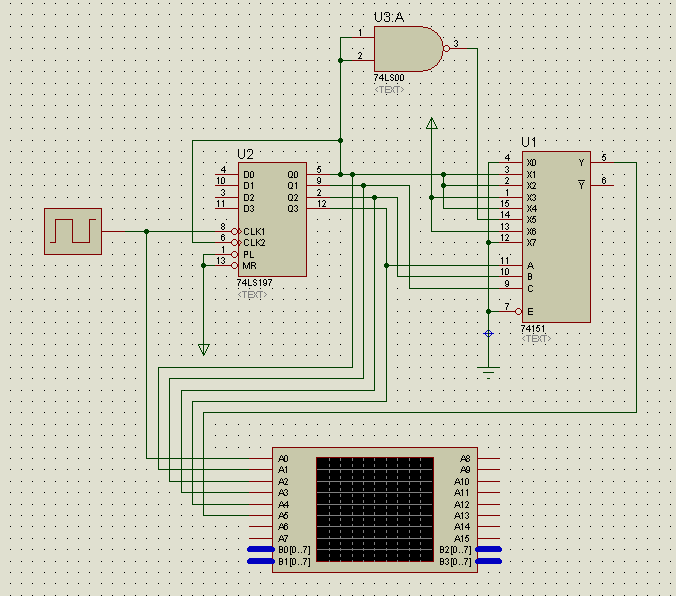
\includegraphics[scale=0.5]{2/2.png}
\end{figure}

\subsubsection{逻辑分析仪}

\begin{figure}[!hbp]
  \centering
  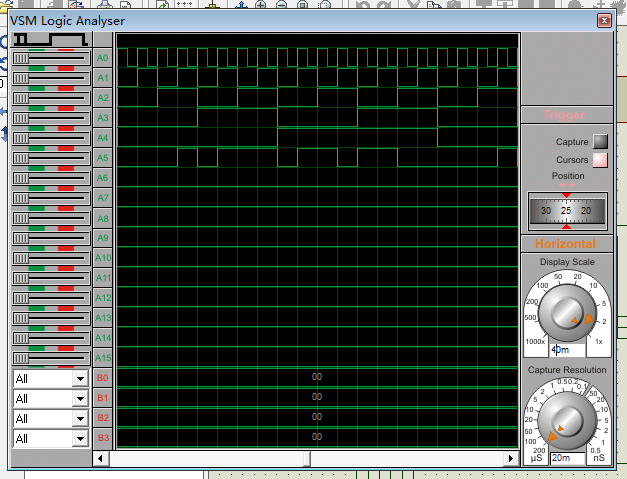
\includegraphics[scale=0.5]{2/1.png}
\end{figure}

\subsection{静态测试}

将输入接到 01 开关,输出接到 01 显示器。

\subsection{动态测试}

\begin{figure}[!hbp]
  \centering
  \includegraphics[scale=0.5]{2/DS2_QuickPrint2.png}
\end{figure}

\subsection{算术单元设计}

\subsubsection{真值表}

\begin{table}[!hbp]
\centering
\begin{tabular}{|c|c|c||c|c|}
\hline
S & A & B & sum & cout \\
\hline
0 & 0 & 0 & 0 & 0\\
\hline
0 & 0 & 1 & 1 & 0 \\
\hline
0 & 1 & 0 & 1 & 0\\
\hline
0 & 1 & 1 & 0 & 1 \\
\hline
1 & 0 & 0 & 0 & 0 \\
\hline
1 & 0 & 1 & 1 & 1\\
\hline
1 & 1 & 0 & 1 & 0 \\
\hline
1 & 1 & 1 & 0 & 0 \\
\hline

\end{tabular}
\end{table}

\subsubsection{表达式}

$sum = \overline{S} \cdot \overline{A}B + \overline{S}A \overline{B} + S \overline{A}B + SA \overline{B}$

$cout = \overline{S}AB + S \overline{A}B$

\subsubsection{电路图}

\begin{figure}[!hbp]
  \centering
  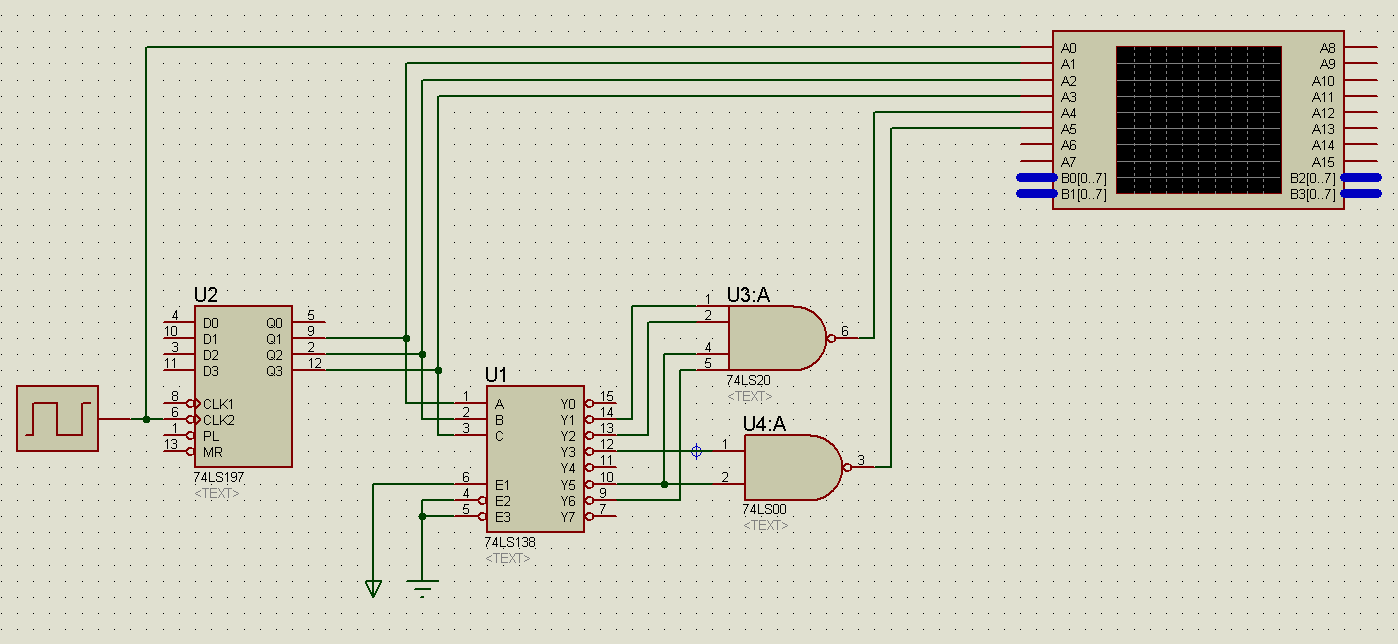
\includegraphics[scale=0.3]{3/1.png}
\end{figure}

\subsubsection{逻辑分析仪}

\begin{figure}[!hbp]
  \centering
  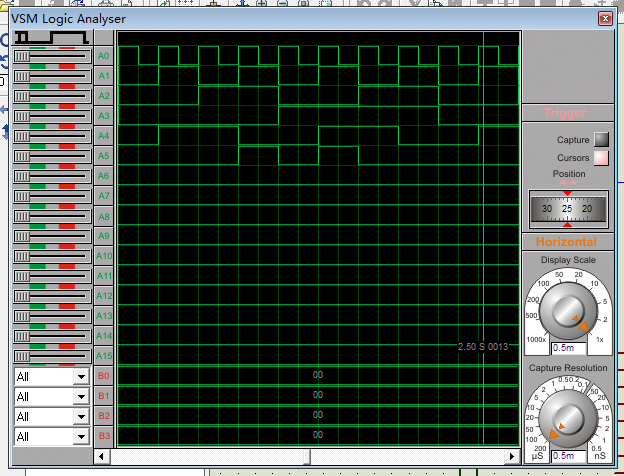
\includegraphics[scale=0.5]{3/2.png}
\end{figure}

\subsection{静态测试}

将输入接到 01 开关,输出接到 01 显示器。

\newpage

\subsection{动态测试}

\begin{figure}[!hbp]
  \centering
  \includegraphics[scale=0.5]{3/DS2_QuickPrint3.png}
\end{figure}

\newpage

\subsection{算术逻辑单元设计}

\subsubsection{电路图}

\begin{figure}[!hbp]
  \centering
  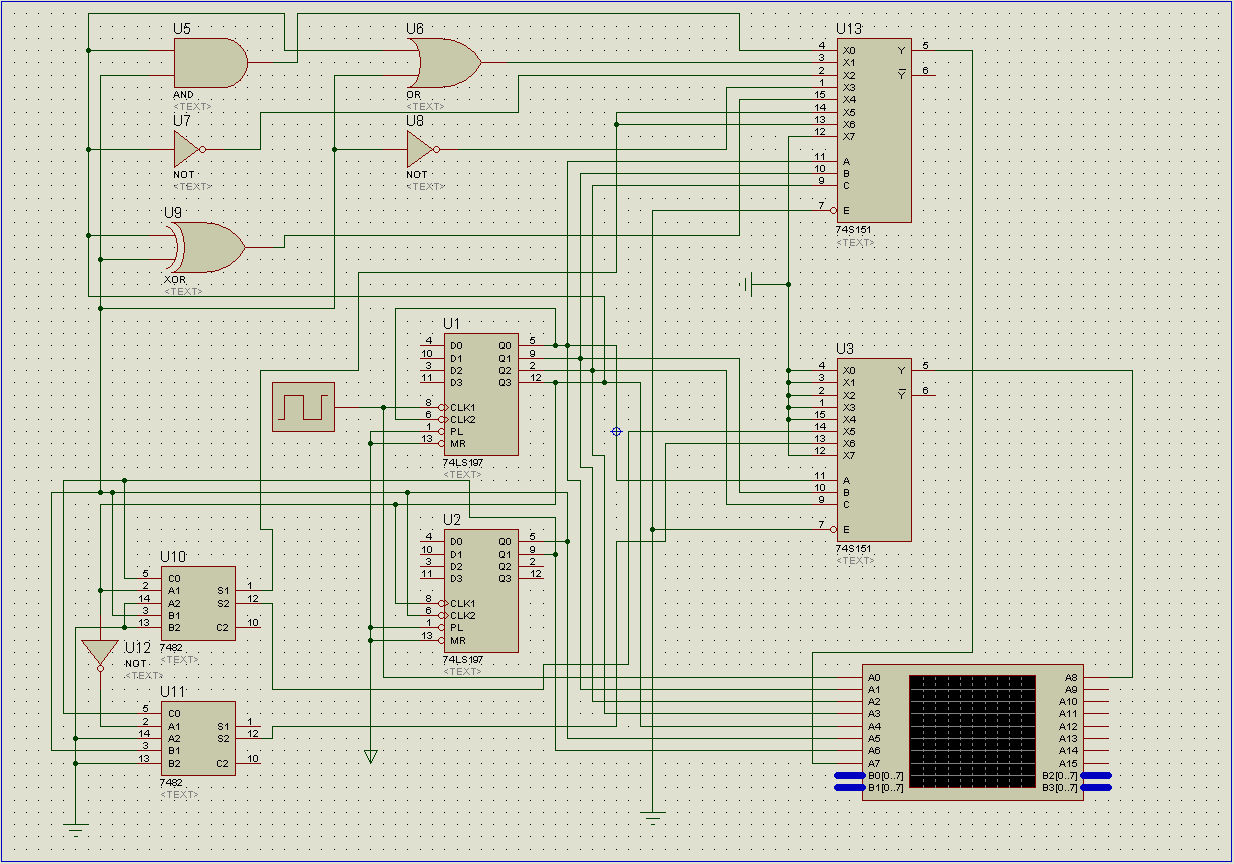
\includegraphics[scale=0.3]{4/1.png}
\end{figure}

\subsubsection{逻辑分析仪}

\begin{figure}[!hbp]
  \centering
  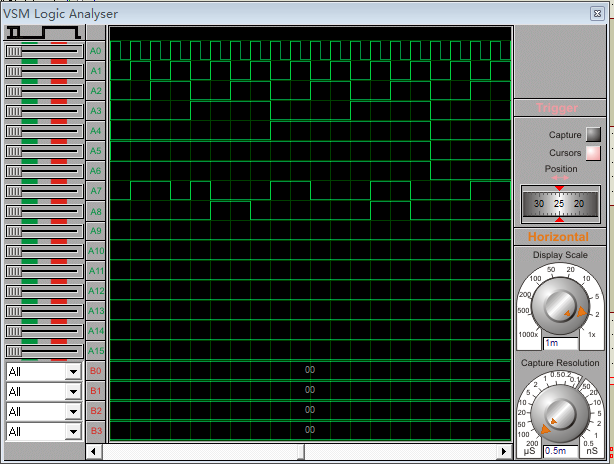
\includegraphics[scale=0.5]{4/2.png}
\end{figure}

\begin{figure}[!hbp]
  \centering
  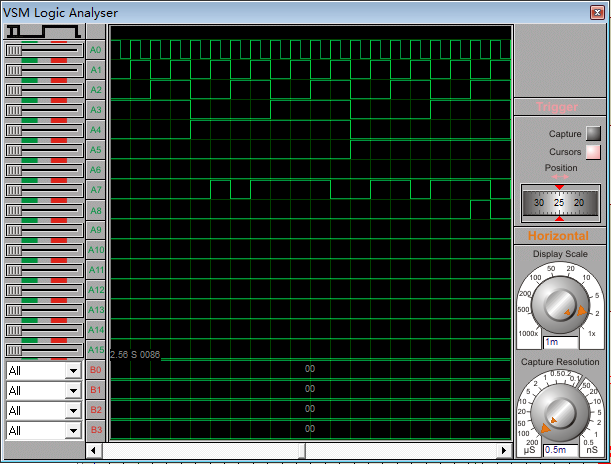
\includegraphics[scale=0.5]{4/3.png}
\end{figure}

\begin{figure}[!hbp]
  \centering
  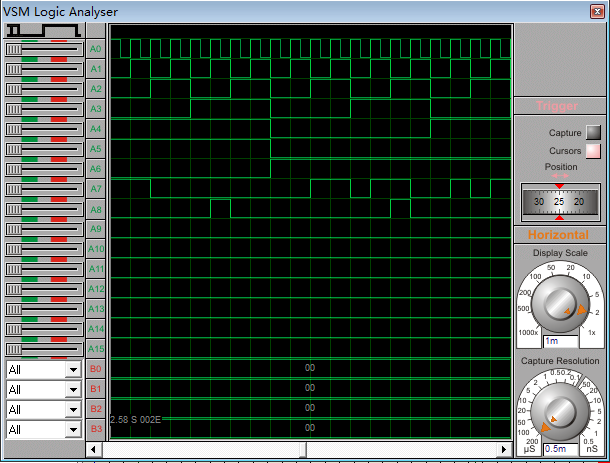
\includegraphics[scale=0.5]{4/4.png}
\end{figure}



\end{document}
















